%%%%%%%%%%%%%%%%%%%%%%%%%%%%%%%%%%%%%%%%%%%%%%%%%%%%%%%%%%%%%%%%%%%%%%%%%%%%%%%
%2345678901234567890123456789012345678901234567890123456789012345678901234567890
%        1         2         3         4         5         6         7         8

\documentclass[letterpaper, 10 pt, conference]{ieeeconf}  % Comment this line out if you need a4paper

%\documentclass[a4paper, 10pt, conference]{ieeeconf}      % Use this line for a4 paper

\IEEEoverridecommandlockouts                              % This command is only needed if 
                                                          % you want to use the \thanks command

\overrideIEEEmargins                                      % Needed to meet printer requirements.

%In case you encounter the following error:
%Error 1010 The PDF file may be corrupt (unable to open PDF file) OR
%Error 1000 An error occurred while parsing a contents stream. Unable to analyze the PDF file.
%This is a known problem with pdfLaTeX conversion filter. The file cannot be opened with acrobat reader
%Please use one of the alternatives below to circumvent this error by uncommenting one or the other
%\pdfobjcompresslevel=0
%\pdfminorversion=4

% See the \addtolength command later in the file to balance the column lengths
% on the last page of the document

% The following packages can be found on http:\\www.ctan.org
\usepackage{graphics} % for pdf, bitmapped graphics files
\usepackage{epsfig} % for postscript graphics files
\usepackage{mathptmx} % assumes new font selection scheme installed
%\usepackage{times} % assumes new font selection scheme installed
% \usepackage{amsmath} % assumes amsmath package installed
% \usepackage{amssymb}  % assumes amsmath package installed
\usepackage{amsmath,amssymb,amsfonts}
\usepackage{url}
\newcommand{\atant}{atan2}
\newcommand*{\QEDA}{\hfill\ensuremath{\blacksquare}}

\newtheorem{theorem}{Theorem}

\usepackage{amsmath,amssymb,amsfonts}
\usepackage{algorithmic}
\usepackage{graphicx}
\usepackage{textcomp}
% \usepackage[linesnumbered,algoruled,boxed,lined,algo2e,ruled,vlined]{algorithm2e}
\usepackage{algorithm,algorithmic}
% links
\usepackage[utf8]{inputenc}
\usepackage[pdftex]{hyperref}
\hypersetup{
    colorlinks=true,
    linkcolor=orange,
    filecolor=magenta,      
    urlcolor=orange,
    pdftitle={Overleaf Example},
    pdfpagemode=FullScreen,
    }

% code
\usepackage{listings}
\usepackage{xcolor}



\definecolor{codegreen}{rgb}{0,0.6,0}
\definecolor{codegray}{rgb}{0.5,0.5,0.5}
\definecolor{codepurple}{rgb}{0.58,0,0.82}
\definecolor{backcolour}{rgb}{0.95,0.95,0.92}

\lstdefinestyle{mystyle}{
    backgroundcolor=\color{backcolour},   
    commentstyle=\color{codegreen},
    keywordstyle=\color{magenta},
    numberstyle=\tiny\color{codegray},
    stringstyle=\color{codepurple},
    basicstyle=\ttfamily\footnotesize,
    breakatwhitespace=false,         
    breaklines=true,                 
    captionpos=b,                    
    keepspaces=true,                 
    numbers=left,                    
    numbersep=5pt,                  
    showspaces=false,                
    showstringspaces=false,
    showtabs=false,                  
    tabsize=2
}

\lstset{style=mystyle}

\title{\LARGE \bf
Recriando uma versão do Flappy Bird com IA}

\author{Moises Souza
\thanks{*Meus agradecimentos}% <-this % stops a space
\thanks{$^{1}$A Deus.
        {\tt\small moises.souza@al.infnet.edu.br}}%
}


\begin{document}

\maketitle
\thispagestyle{empty}
\pagestyle{empty}


%%%%%%%%%%%%%%%%%%%%%%%%%%%%%%%%%%%%%%%%%%%%%%%%%%%%%%%%%%%%%%%%%%%%%%%%%%%%%%%%
% Abstract
%

%%%%%%%%%%%%%%%%%%%%%%%%%%%%%%%%%%%%%%%%%%%%%%%%%%%%%%%%%%%%%%%%%%%%%%%%%%%%%%%%
% Sections
%
\section{Introdução}\label{sec:intro}
A Natureza sempre serviu de inspiração para diversas áreas, no campo artístico temos pintores, poetas e na arquitetura podemos citar a resolução do problema do \textbf{Trem-bala} do \textbf{Japão}. A solução do problema foi encontrada por \textbf{Eiji Nakatsu}, engenheiro e observador de pássaros, tentando contornar o problema da poluição sonora e a explosão sônica, ele teve a ideia de  imitar a aerodinâmica do pássaro \textbf{Martim-pescador (um espécie pássaro)}.  A ave, que precisa mergulhar para se alimentar, troca rapidamente de um ambiente de baixa resistência (ar) para um com muita resistência (água), ela possui a aerodinâmica perfeita para essa situação. Por isso o Trem-bala foi inspirado nesta ave\cite{area_engenaria} Na tecnologia da informação (TI) não é diferente, tivemos \textbf{Alan Kay}, ele era matemático, biólogo, criou o paradigma de orientação a objetos.  O matemático, formulou sua "analogia algébrico-biológica". \textbf{Kay}, lançou o postulado de que segundo ele, “o computador ideal deveria funcionar como um organismo vivo, isto é, cada célula se relaciona com outras a fim de alcançar um objetivo, mas cada uma funciona de forma autônoma. As células poderiam também reagrupar-se para resolver outro problema, ou desempenhar outras funções”.\cite{Alan_Kay}
Em virtude disso, o conhecimento das unidades principais do cérebro, conhecidas como os neurônios, estabelecem explicações para iniciar a compreensão deste estudo.
\cite{Neuronio}.
  O funcionamento do cérebro consiste em desenvolve suas regras através da experiência adquirida em situações vividas anteriormente\cite{Neuronio}.
A busca pelo desenvolvimento de um programas que realize funções da mente humana
começou logo  partir de 1930, começam as pesquisas para substituir as partes mecânicas por elétricas, como exemplo o \textbf{Mark I} (A Calculadora Automática de Seqüência Controlada), concluído em 1944\cite{uff}. Desde então, muitas pesquisas foram
feitas para chegar a este objetivo. Na tentativa, surgem modelos computacionais interessantes, dentro da grande área de Inteligência Artificial.
As Redes Neurais Artificiais, também designadas neste trabalho por RNA, que são inspiradas no funcionamento do cérebro humano que usa uma abstração matemática do neurônio biológico denominada de perceptron.\cite{MCCULLOCH}
Com a redução do custo de equipamentos utilizados
para processar redes neurais, oportunizam a execução de algoritmos de aprendizado em
computadores pessoais e dando novo fomento ao desenvolvimento de novos algoritmos, e softwares que utilizam \textbf{RNA}.
As Redes neuronais artificiais são modelos computacionais inspirados pelo sistema nervoso central, eles são capazes de realizar o aprendizado de máquina, bem como o reconhecimento de padrões,  para criar esses modelos ou métodos avançados  requer um grande conhecimento matemático e demanda de muito tempo. Tendo em vista que hoje focamos no desenvolvimento de software ágil, seria contraproducente perder muito tempo no desenvolvimento desses modelos do zero.
Porém, com o surgimento das bibliotecas, TensorFlow, Keras e Neat-pytho,	
esse processo se torna muito mais fácil e nos ajuda a construir e implementar facilmente  modelos de aprendizagem de máquina. Neste projeto usarei o
Neat-python.
O NEAT, que tem como objetivo criar uma rede neural artificial que evolui através de mudança em sua delineação e alteração de pesos das suas conexões, seguindo a abordagem de algoritmos neuroevolutivos.
O \textbf{NEAT} é um algoritmos de neuroevolução que melhora o desempenho da arquiteturas de rede neural.
Este trabalho consiste em utilizar a \textbf{programação Orientada a objeto (POO)} a biblioteca \textbf{NEAT-PYTHON} para evolução de redes neurais arbitrárias, tendo como foco
criar o jogo \textbf{Flappy Bird}, por ser um jogo simples e de fácil implementação, facilitando a compreenção de algoritmos de neuroevolução para melhorar o desempenho de arquiteturas de rede neural.
Os objetivos específicos deste trabalho são: \break 
\begin{itemize}
    \item Estudar conceitos básicos
de evolução de redes neurais;\\
     \item Mapear soluções de software pré-existentes para a montagem do sistema de aprendizado de neuroevolução;\\
     \item Utilizarar a biblioteca do NEAT-python para a criação do jogo Flappy Bird.\\
     \item Avaliar os resultados obtidos e discutir sobre seu desempenho.
\end{itemize} 


 
\section{Bases teóricas}\label{sec:theory}
Nesta seção abordarei os principais conceitos necessários para o desenvolvimento do trabalho, formalizando o suporte para que as próximas etapas sejam construídas com uma
linguagem de nível mais alto demonstrando os conceitos do:\\ \textbf{POO, Neat-Python, Pygame, Python}.
\subsection{Redes Neusrais}
Redes neurais artificiais significa \textbf{( RNA )} um grafo de nós conectados por links em que cada um dos links tem um peso específico.
Nos últimos 70 anos, muitos métodos de treinamento de \textbf{RNA} foram propostos, porém, a técnica mais popular que ganhou fama nesta década foi proposta por \textbf{Jeffrey Hinton}.\cite{rna} É baseado na retropropagação do erro de predição através da rede, com várias técnicas de otimização construídas em torno da descida do gradiente da função de perda, em relação aos pesos de conexão entre os nós da rede. Ele demonstra o excelente desempenho do treinamento de redes neurais profundas para tarefas relacionadas principalmente ao reconhecimento de padrões.
 No entanto, existe um \textbf{trade-off}, ele tem desvantagens  e desvantagens:
\begin{itemize}
    \item Grande quantidade de amostras de treinamento para aprender algo útil de um conjunto de dados específico.\\
     \item Arquitetura de rede fixa criada manualmente pelo desenvolvedor, o que resulta no uso ineficiente de recursos computacionais. Isso se deve a uma quantidade significativa de nós da rede que não participam do processo de inferência. \\
     \item Os métodos baseados em retropropagação têm problemas com a transferência do conhecimento adquirido para outros domínios semelhantes.\\
    
\end{itemize} 
O conceito de redes neurais artificiais ( RNA ) foi\\ inspirado na estrutura do cérebro humano. Havia uma forte crença de que, se pudéssemos imitar essa estrutura emaranhada de uma forma muito semelhante, seríamos capazes de criar inteligência artificial. Ainda estamos engatinhando para alcançá-lo, embora possamos implementar agentes AI,  ainda estamos longe de criar um agente de AI genérico. Além dos métodos de retropropagação, também existem algoritmos evolutivos que prometem muito e que podem resolver os problemas mencionados. Essas técnicas inspiram-se na teoria da evolução de Darwin e usam abstrações de evolução natural para criar redes neurais artificiais.
Para obter mais informações sobre os assuntos mencionados.\cite{Neural_Network_V4}\cite{Neural_Network_V6}

\subsection{\textbf{Neuroevolução}}
\begin{itemize}
    \item A neuroevolução consiste em produzir as RNAs usando métodos de pesquisa estocásticos baseados em populações. É possível desenvolver arquiteturas ótimas de redes neurais, que cuidam com precisão dessas  tarefas específicas usando o processo evolutivo.
O resultado disso são redes compactas e moderadamente eficientes em termos de energia computacional. O processo evolutivo é executado pela aplicação de operadores genéticos\textfb{( mutação , cruzamento)} para a população de cromossomos (representações geneticamente codificadas de \extbf{NAs}/ sluções) ao longo de muitas gerações. A crença central é que, se tornarão melhores aproximadores da função objetivo.\cite{neuroevolucao}
\end{itemize}

%
%%%%%%%%%%%%%%%%%%%%%%%%%%%%%%%%%%%%%%%%%%%%%%%%%%%%%%%%%%%%%%
%
\subsection{\textbf{Teoria complementar}}\label{sec:ANN}
%
Abordaremos os conceitos básicos de algoritmos evolucionário, e como eles diferem-se dos algoritmos convencionais, que usam métodos baseados em retropropagação de erro para treinar a RNA.
Abordarei um pouco sobre algoritmo genético, 
para entender melhor o processo como um todo: 
\begin{itemize}
\item {\bfseries {Operadores genéticos}}
\begin{itemize}
    \item \emph{ Os operadores genéticos são o ponto central de todo algoritmo evolucionário, e o desempenho de qualquer algoritmo neuroevolucionário  desses pontos. Existem dois principais operadores genéticos são:}
                \begin{itemize}
                    \item mutação.
                    \item cruzamento (recombinação).
                \end{itemize}
\end{itemize}
\item {\bfserie{Operador de mutação}}
\begin{itemize}
    \item \emph{O operador de mutação tem um papel essencial de preservar a diversidade genética da população durante a evolução e evita estagnação nos mínimos locais quando os cromossomos dos organismos em uma população se tornam muito semelhantes.
    A mutação altera um ou mais genes do cromossomo, de acordo com a probabilidade de mutação definida pelo desenvolvedor. Ao introduzir mudanças aleatórias no cromossomo do solucionador, a mutação permite que o processo evolutivo explore novas áreas no espaço de busca de soluções possíveis e encontre soluções cada vez melhores ao longo das gerações.}
\end{itemize}

\item {\textbf{Operador de cruzamento}}
\begin{itemize}
    \item \emph{Com o cruzamento (recombinação) podemos gerar estocasticamente novas gerações (soluções) a partir de populações existentes por meio da recombinação de informações genéticas de dois pais para gerar proles. Assim, as porções de boas soluções de organismos pais podem ser combinadas e podem potencialmente levar a uma prole melhor. Normalmente, após um cruzamento, a prole produzida sofre mutação antes de ser adicionada à população da próxima geração.}\\
\end{itemize}

\begin{center}
    \textbf{#Processo de execução em ordem}
\end{center}
\item {\textbf{Geramos a população}}
\begin{itemize}
    \item \emph{A população é gerada aleatoriamente e pode ser utilizado um método randômico da geração da população inicial.\\}
\end{itemize}

\item {\bfseries Avaliamos a população}
\begin{itemize}
    \item \emph{A avaliação consiste em testar a aptidão dos indivíduos dessa população.
Assim saberemos quais são os melhores indivíduos.
para depois selecioná-los.
}
\end{itemize}
\item {\bfseries Selecionamos os melhores}
\begin{itemize}
    \item \emph{após a avaliação de cada indivíduos da população selecionamos através do métodos de seleção que será usado para determinar qual dos indivíduos da população conseguirá se reproduzir e criar os descendentes que formará a próxima geração.\\ O método de seleção consiste em selecionar aqueles indivíduos com valores de pontuação mais altos esses têm maior probabilidade de serem selecionados e passarem seu material genético para a próxima geração. Indivíduos com baixos valores de aptidão ainda podem ser selecionados, mas com menor probabilidade. Dessa forma, seu material genético não é totalmente excluído.}\\
\end{itemize}
\item {\bfseries Aplicamos o Crossover para gerar descendentes}
\begin{itemize}
    \item \emph{Para criar um par de novos indivíduos, são escolhidos dois indivíduos da geração atual e partes de seus cromossomos são trocadas (cruzadas) para criar dois novos cromossomos que representam descendentes. Esta operação é chamada de crossover ou recombinação}\\
\end{itemize}
\item {\bfseries E aplicamos a mutação aos descendentes}
\begin{itemize}
    \item \emph{O objetivo da mutação é atualizar a população periódica e aleatoriamente , introduzir novos padrões nos cromossomos e encorajar a pesquisa em áreas não mapeadas no hiperplano da solução.
Uma mutação pode ser alterada aleatoriamente em um gene. As mutações são feitas como mudanças aleatórias em um ou mais dos valores cromossômicos.
}\\
\end{itemize}
\end{itemize}
\textfb{Também precisamos levantar alguns pontos como}:
\begin{itemize} 
\item Variáveis necessárias:\\
Quantos Neurônio são necessário para modelar esse hiperplano...
\begin{itemize}
\item Vai depender da complexidade do seu problema! 
\end{itemize}
\item Tempo de convergência:\\
Mais neurônios afetaria diretamente o tempo de convergência da aplicação.\\  
A busca é por uma convergência rápida, sem custo computacional desnecessário\\
\item Arquitetura:\\
É suma importância modelar uma arquitetura boa para resolver o problema. 
Este é o momento de pensar na quantidade exata de variáveis a ser usada
e levantar os impactos que pode causar.
    \begin{itemize}
\item O que são arquitetura de redes neurais:\\
Falando de arquitetura de uma rede neural estamos nos referindo sobre a disposição dos neurônios, um em relação ao outro, seguindo as conexões sinápticas comentadas.\\
Veja a primeira imagem dessa rede neural, ela é uma rede neural do tipo Fully Connected
ela tem dois neurônios na camada de entrada, dois camada oculta e um neurônio na camada de saída totalmente conectados,
e a segunda imagen é bem mais simples, mas também é uma rede  neural  do  tipo  Fully  Connected.\\
A complexidade de uma arquitetura pode influenciar no tempo de convergência. \cite{arquiteturaRN}
\begin{center}
    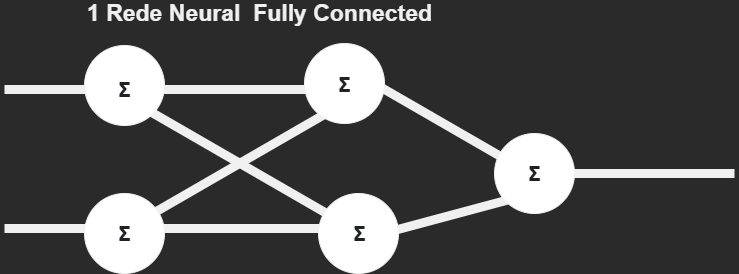
\includegraphics[width=7cm]{images/1_RN_FULLY CONNECTED.png}\break
    
\end{center}
\begin{center}
    
     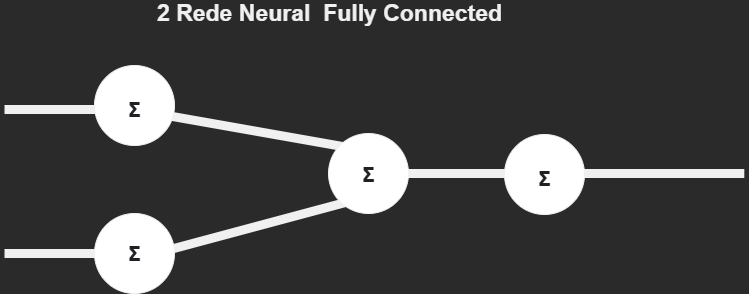
\includegraphics[width=7cm]{images/2_RN_FULLY CONNECTED.png}\break
\end{center}

    \end{itemize}
    

\end{itemize}




 
%
%%%%%%%%%%%%%%%%%%%%%%%%%%%%%%%%%%%%%%%%%%%%%%%%%%%%%%%%%%%%%%
%
\subsection{Pygame}\label{sec:ANN}

Pygame é um conjunto de plataforma cruzada de módulos Python que é usado para criar videogames.
Consiste em computação gráfica e bibliotecas de som projetadas para serem usadas com a linguagem de programação Python.
Pygame foi oficialmente escrito por Pete Shinners para substituir PySDL.
Pygame é adequado para criar aplicativos do lado do cliente que podem ser potencialmente agrupados em um executável autônomo.
O seu nome tem origem da junção de Py, proveniente de Python e Game, que significa Jogo, ou seja, Jogos em Python.
Gênero(s): Motor de jogo
Idioma(s): inglês
Licença: LGPL
Versão estável: 2.0.1 (24 de dezembro de 2009)
Linguagens de programação: Python, C, Cython, Linguagem assembly\cite{pygame_info_wikipedia}


\subsection{Python}\label{sec:ANN}
Python é uma linguagem de programação interpretada, orientada a objetos e de alto nível Tem ocupado o primeiro lugar no índice do TIOBE no ano de 2021.
O índice da comunidade de programação TIOBE é um indicador da popularidade das linguagens de programação, e pode ser usado como termômetro e um guia para tomada de decisão estratégica sobre qual linguagem de programação deve ser adotada ao iniciar a construção de um novo sistema de software.
As classificações são baseadas no número de engenheiros qualificados em todo o mundo, cursos e fornecedores terceirizados, motores de busca populares como Google, Bing, Yahoo, Wikipedia, Amazon, YouTube e Baidu são usados ​​para calcular as classificações.
O índice do TIOBE não trata da melhor linguagem e sim a mais popular entre os engenheiros e motores de busca da internet.
\cite{tiobe} Python e a extensa biblioteca padrão estão disponíveis em formato de código-fonte ou binário gratuitamente para todas as principais plataformas e podem ser distribuídos gratuitamente.. Foi lançada por Guido van Rossum em 1991
Criado Por: Guido van Rossum
Empresa matriz: Python Software Foundation\cite{python_info_wikipedia}.

\subsection{\textbf{Visão geral do NEAT}}\label{sec:ANN}
%
NEAT é um método desenvolvido por Kenneth O. Stanley para a evolução de redes neurais arbitrárias. NEAT-Python é uma implementação em Python pura do NEAT, sem dependências além da biblioteca padrão do Python.\\
São algoritmos baseados na biologia humana
os quais se utilizam de estrutura chamadas de neurônios 
agrupados para formar uma nova estrutura chamada de rede neural artificial
e esses neurônios são como variáveis para modelar um hiperplano,
que precisa ser modelado para encaixar numa equação a qual descreva seu problema.\\ 
Também devemos abordar sobre aprendizado, pois é por ele que o hiperplano é modelado,
citarei três maneiras de aprendizado porém focaremos na terceira e última, pois é o que dá base para neuroevolução e NEAT.\\
		
		
{\bfseries Aprendizado:}

\begin{itemize}

\item Aprendizado Supervisionado 
\item Aprendizado não-Supervisionado 
\item Aprendizado por Reforço:
\begin{itemize}
\item \emph{A aprendizagem por reforço lida com os conceitos de recompensas e
penalidades. O objetivo dessa modalidade é escolher um conjunto de ações que
maximize as recompensas}
\end{itemize}
\end{itemize}

%






 
\section{Metodologia}\label{sec:methods}

Este Trabalho foi desenvolvido através de pesquisa bibliográfica que fornece subsídios
para empreender as análises referentes à necessidade de implementação de um modelo de
científicos. Nesta pesquisa, quanto aos objetivos, caracteriza-se como descritiva\cite{GIL}
, identificando os possíveis benefícios, funcionalidades e contribuições do
Sistema de Informações, aborda o processo formal e sistemático de desenvolvimento do método científico, sendo seu objetivo fundamental a obtenção de respostas para questões mediante o emprego de procedimentos científicos.Além disso, Segundo \cite{GIL}, “a pesquisa bibliográfica é elaborada com base em material
já publicado”, incluindo [...] “livros, revistas, jornais, teses, dissertações e anais de eventos
científicos”. A pesquisa bibliográfica permite elaborar as informações científicas já existentes,

sistematizando o conhecimento já produzido\cite{LEHFELD} 
 Tendo em vista que a Neuroevolução é uma forma de aprendizado de inteligência artificial,  e consiste em utilizada com algoritmos evolutivos para  melhorar o desempenho de arquiteturas de rede neural, simplificar o processo de resolução de tarefas complexas em domínios como jogos, robótica e simulação de processos naturais.\cite{neuroevolucao}
À partir dessa informação, tem como foco mostrar os conceitos que foram usados para o recriação de um jogo já existente denominado de Flappy Bird, é um jogo eletrônico criado para dispositivos móveis desenvolvido no ano  de 2013 desenvolvido em Hanói Capital do Vietnã, Pelo DESENVOLVEDOR vietnamita Nguyễn Hà Đông e publicado pela .GEARS studios.\cite{CriadorJogo}

A ideia restringe se em recriar o jogo Flappy Bird utilizando \textbf{NEAT} para fazer com que o Agente aprenda sozinho como jogar e zerar o jogo vencendo todas as fases e passando por todos os obstáculos. a escolha do jogo nasceu por ser um jogo simples e de fácil e de rápida criação podendo assim aplicar as técnicas de criação da interface com o Pygame 
Na fase inicial eu utilizei o Pygame  para construir a parte gráfica cálculos de  Largura e Altura de tela e iniciação de fonte  desenho dos elementos em tela. e iniciação de fonte  desenho dos elementos em tela.
Utilização da programação orientada a objetos para criação dos elementos do jogo 
que é o pássaro, cano e chão.
O objeto pássaro é composto de imagens para fazer a animação do bater das asas
\textbf{Contém quatro funções:}
\begin{itemize}
    \item \textbf{Init}
    \begin{itemize}
    \item A função \textbf{init} que é chamada na instanciação do objeto recebendo como parâmetros 
os valores de X e Y que determinam as coordenadas do objeto pássaro no plano cartesiano, dados que vão ser passados para minha rede para tomada de decição do agente.
\end{itemize}


\item \textbf{jump}
    \begin{itemize}
    \item A função Jump controla os valores de velocidade e tempo controlando a variação, e atribui a altura o valor da variável \textbf{Y (Variável que representa o eixo de subida)}  
\end{itemize}

 

\item \textbf{Move}
    \begin{itemize}
    \item A função Move que determina o movimento que consiste em um função MRUV para determinar o deslocamento.\\
S = so + vot + at²/2
 \textbf{Y}
\end{itemize}

\item \textbf{draw}
    \begin{itemize}
    \item A função draw faz animação do bater de asas desenhar a pássaro na tela, através de uma função screen.blit objeto passada por parâmetro na função draw.
\end{itemize}
\end{itemize}

as outras são iniciadas com valores padrão e imagens carrega com um array de imagens para compor a animação do pássaro








%
\subsection{\textbf{Implementação da IA com Neat-Python}}
Vamos analisar a parte dos hiperparâmetros que fica no arquivo \textbf{config.txt}.
A parte mais importante são os parâmetros de rede,
que representa o nosso perceptron ilustrado na imagem abaixo.
Os num inputs são os sensores do agente, onde vai
perceber o ambiente, \textbf{a posição do agente no eixo Y + distância do agente para o cano de cima + distância do pássaro para o cano de baixo = num inputs = 3}, são as informações que vou colocar na rede, 
que no meu caso são 3.
E meu num outputs = 1 pois ação do meu agente é saltar
O parâmetro num hidden = 0 , ele seria o número de camada oculta no entanto isso você aumenta a complexidade da sua rede resultando uma em um tempo maior de convergência falaremos disso em resultado e teste. 
\begin{lstlisting}
# network parameters
num_hidden              = 0
num_inputs              = 3
num_outputs             = 1
\end{lstlisting}

\begin{figure}[htpb!]
    \centering 
    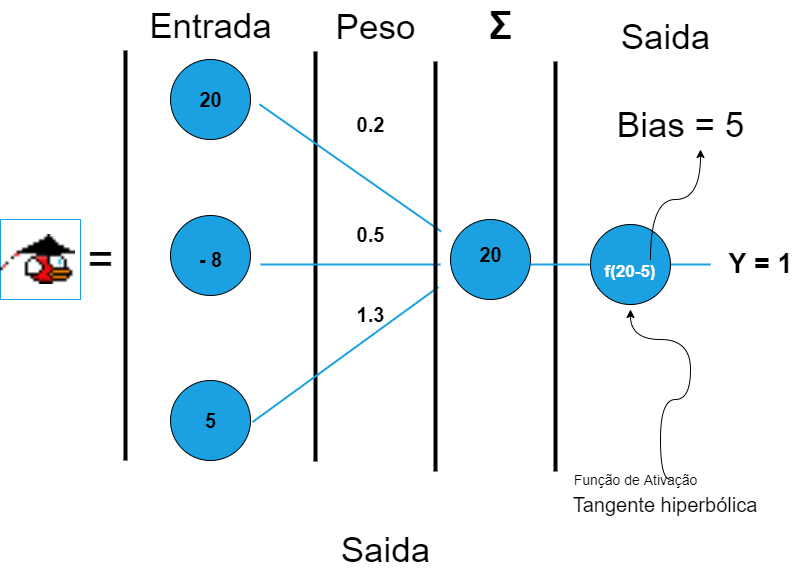
\includegraphics[width=0.7\linewidth]{images/passaroRNA3.png}
    \caption{Perceptron.}
    \label{fig:gym}
\end{figure}
O projeto a qual me inspirei  num imputs = 5 sensores do carro e
num outputs  = 3, pois há 3 ações. virar a esquerda, virar a direita, e aceleração.
O parametro num hidden = 0.
\begin{figure}[htpb!]
    \centering 
    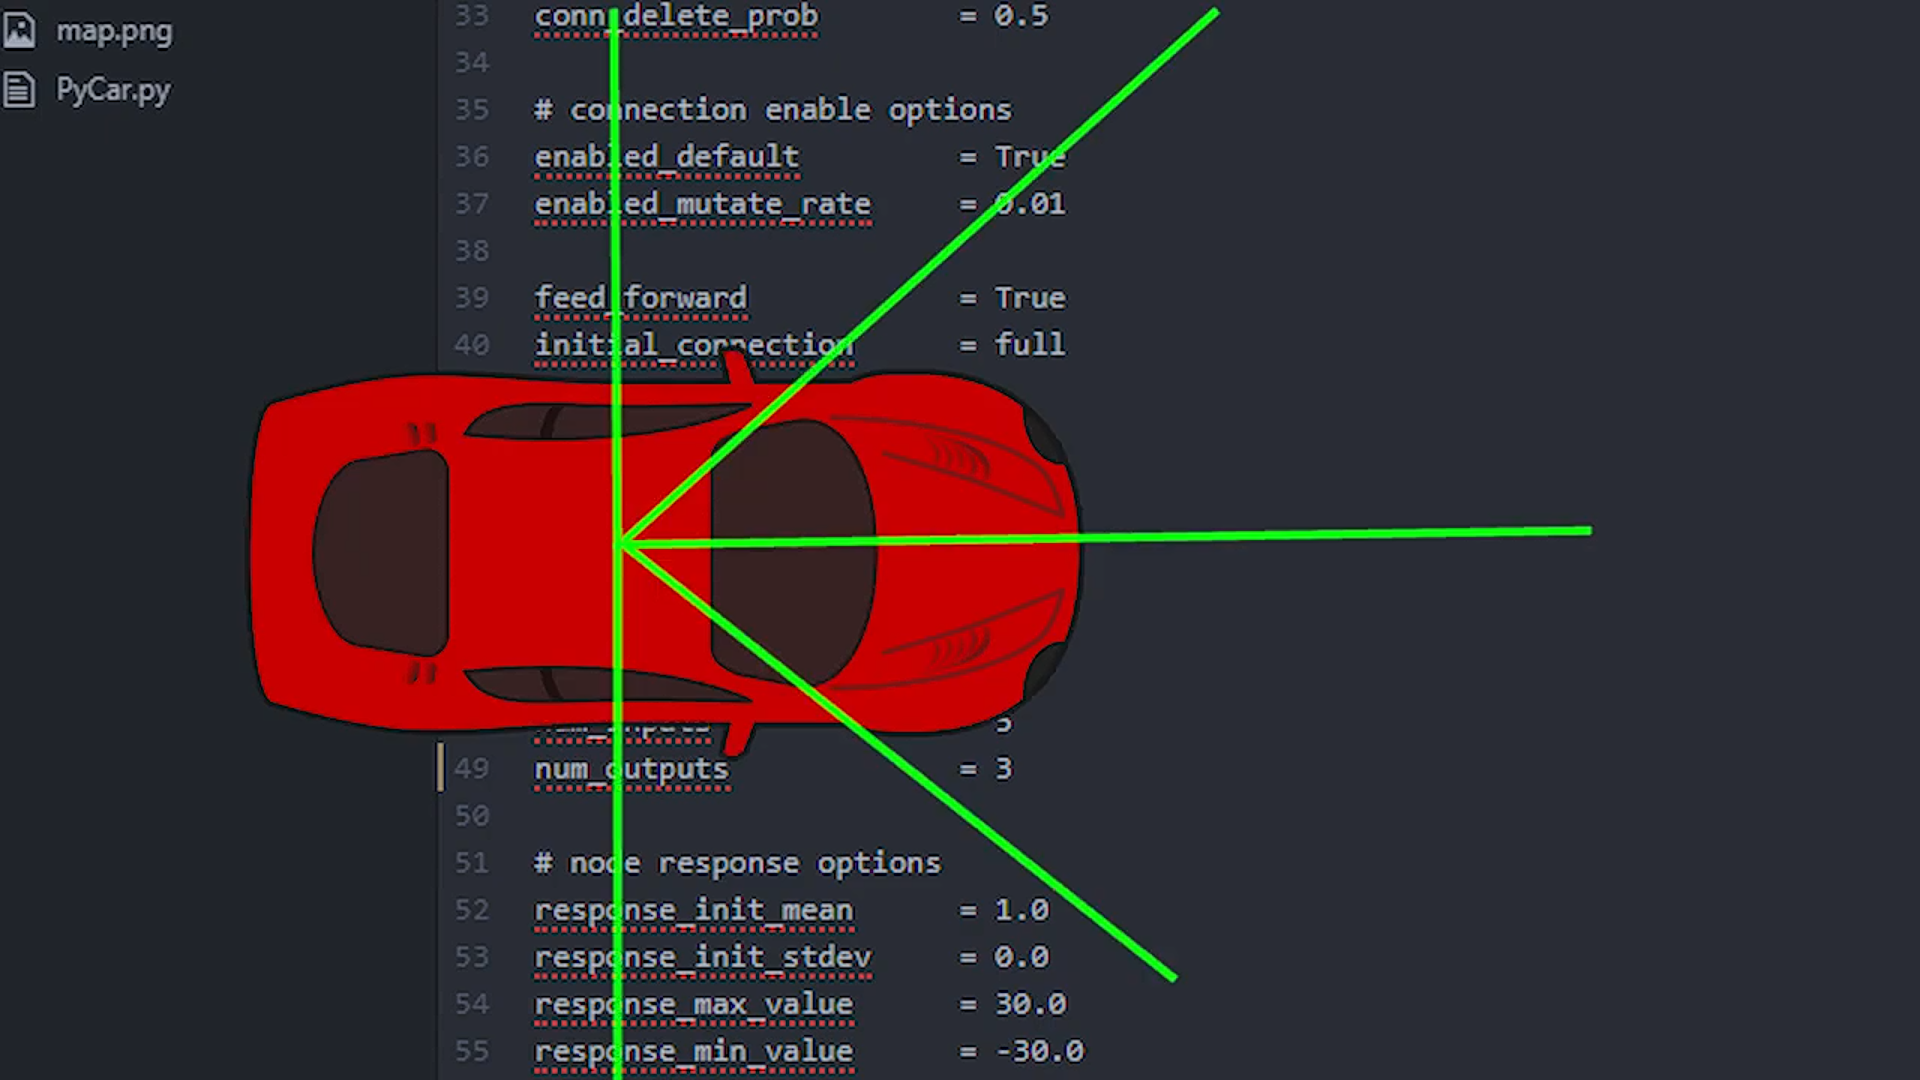
\includegraphics[width=0.7\linewidth]{images/car.png}
    \caption{project the reference channel Cheesy AI.}
    \label{fig:gym}
\end{figure}
\cite{Cheesy}

abaixo você pode encontra uma referência para mais informações. \textbf{config.txt}
\begin{lstlisting}[language=Python, caption=Detalhes de implementação do arquivo → \href{https://neat-python.readthedocs.io/en/latest/config_file.html}{config.txt} 
  \cite{neat-python}]
[NEAT]
fitness_criterion     = max
fitness_threshold     = 1000
pop_size              = 100
reset_on_extinction   = False

[DefaultGenome]
# node activation options
activation_default      = tanh
activation_mutate_rate  = 0.0
activation_options      = tanh

# node aggregation options
aggregation_default     = sum
aggregation_mutate_rate = 0.0
aggregation_options     = sum

# node bias options
bias_init_mean          = 0.0
bias_init_stdev         = 1.0
bias_max_value          = 30.0
bias_min_value          = -30.0
bias_mutate_power       = 0.5
bias_mutate_rate        = 0.7
bias_replace_rate       = 0.1

# genome compatibility options
compatibility_disjoint_coefficient = 1.0
compatibility_weight_coefficient   = 0.5

# connection add/remove rates
conn_add_prob           = 0.5
conn_delete_prob        = 0.5

# connection enable options
enabled_default         = True
enabled_mutate_rate     = 0.01

feed_forward            = True
initial_connection      = full

# node add/remove rates
node_add_prob           = 0.2
node_delete_prob        = 0.2

# network parameters
num_hidden              = 0
num_inputs              = 3
num_outputs             = 1

# node response options
response_init_mean      = 1.0
response_init_stdev     = 0.0
response_max_value      = 30.0
response_min_value      = -30.0
response_mutate_power   = 0.0
response_mutate_rate    = 0.0
response_replace_rate   = 0.0

# connection weight options
weight_init_mean        = 0.0
weight_init_stdev       = 1.0
weight_max_value        = 30
weight_min_value        = -30
weight_mutate_power     = 0.5
weight_mutate_rate      = 0.8
weight_replace_rate     = 0.1

[DefaultSpeciesSet]
compatibility_threshold = 3.0

[DefaultStagnation]
species_fitness_func = max
max_stagnation       = 20
species_elitism      = 2

[DefaultReproduction]
elitism            = 2
survival_thr
\end{lstlisting}
Abstração da implementação do projeto com Neat-Python
\begin{figure}[htpb!]
    \centering 
    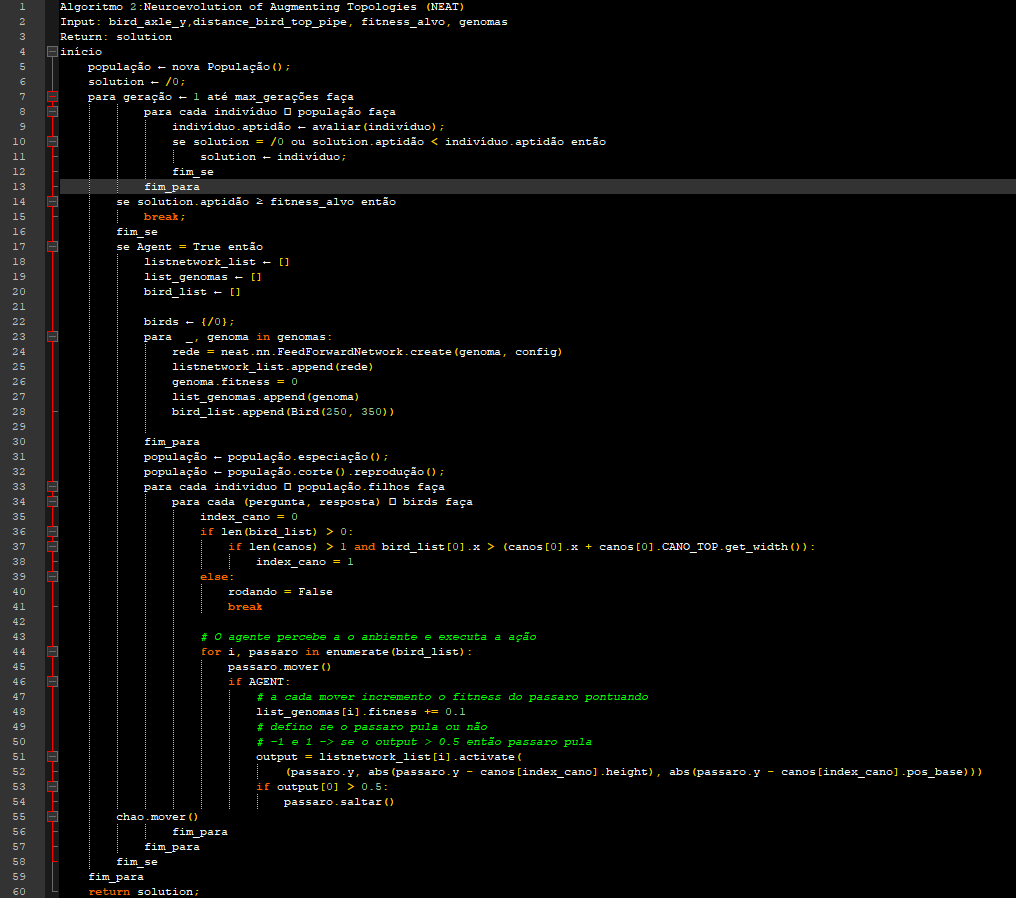
\includegraphics[width=0.7\linewidth]{images/abstract.png}
    \caption{abstração do projeto com Neat-Python}
    \label{fig:gym}
\end{figure}\\
Referência para detalhes do código 
\cite{mygit}
  

%



 
\section{Simulação e Resultados}\label{sec:experimental}
%

##População inicial, primeiros indviduos gerado##
\begin{figure}[htpb!]
    \centering 
    \includegraphics[width=4cm\linewidth]{images/1g_pt0.png}
    
    \caption{Primeira geração.}
    \label{fig:gym}
\end{figure}
\subsection{\textbf{Primeira etapa de teste}}
Nesta etapa de teste foi gerado 100 indivíduos (Redes Neurais)
com 3 entradas e uma saída não tendo camada oculta
a primeira geração a aptidão média da população foi de: 4.56600 
O melhor indivíduo  apto um fitness de: 45,60000 com tamanho: (1, 3)
Primeira espécie de : id 10.
Aptidão média foi ajustada para: 0,050.
A distância genética média é de 1,126, com desvio padrão 0,476.
Uma rede de baixa complexidade um tempo de convergência de 10.764s
O resultado esperado já foi alcançado na segunda geração. 
Com a população de 50 membros em 1 espécie:

\begin{lstlisting}

 ID   age  size  fitness  adj fit  stag
  ====  ===  ====  =======  =======  ====
     1    0    50     45.6    0.050     0

\end{lstlisting}
\begin{figure}[htpb!]
    \centering 
    \includegraphics[width=0.6\linewidth]{images/2g_pt2.png}
    \caption{Segunda Geração.}
    \label{fig:gym}
\end{figure}
%

  
\subsection{\textbf{Segunda etapa de teste}}
Nesta etapa de teste foi gerado 100 indivíduos (Redes Neurais)
com 3 entradas e uma saída com 2 camadas ocultas
a primeira geração a aptidão média da população foi de: 4.45400 
O melhor indivíduo  apto um fitness de: 20.10000 com tamanho: (3, 8)
Terceira espécie de : id 3.
Aptidão média foi ajustada para:0.116.
A distância genética média é de 3.251, com desvio padrão 0.504.
Uma rede de uma alta complexidade obteve um tempo de convergência de 5.597 sec na sua primeira Geração.
O resultado esperado não foi alcançado. 
Com a população de 100 membros em 50 espécie:
\begin{lstlisting}

 ID   age  size  fitness  adj fit  stag
  ====  ===  ====  =======  =======  ====
     1    0     2      2.4    0.000     0
     2    0     2      7.6    0.294     0
     3    0     2     20.1    1.000     0
     4    0     2      2.4    0.000     0
     5    0     2      2.5    0.006     0
     6    0     2      2.4    0.000     0
     7    0     2      2.6    0.011     0
     8    0     2      2.4    0.000     0
     9    0     2      2.5    0.006     0
    10    0     2      3.9    0.085     0
    11    0     2      2.4    0.000     0
    12    0     2      2.5    0.006     0
    13    0     2      8.1    0.322     0
    14    0     2      7.5    0.288     0
    15    0     2      3.9    0.085     0
    16    0     2      2.4    0.000     0
    17    0     2      4.0    0.090     0
    18    0     2      2.4    0.000     0
    19    0     2      7.6    0.294     0
    20    0     2      2.4    0.000     0
    21    0     2      3.9    0.085     0
    22    0     2      3.7    0.073     0
    23    0     2      2.4    0.000     0
    24    0     2      2.5    0.006     0
    25    0     2      2.4    0.000     0
    26    0     2      2.6    0.011     0
    27    0     2      7.5    0.288     0
    28    0     2      3.9    0.085     0
    29    0     2      2.4    0.000     0
    30    0     2      2.5    0.006     0
    31    0     2      7.7    0.299     0
    32    0     2      7.5    0.288     0
    33    0     2      7.6    0.294     0
    34    0     2      2.4    0.000     0
    35    0     2      2.5    0.006     0
    36    0     2      2.4    0.000     0
    37    0     2      3.9    0.085     0
    38    0     2      8.0    0.316     0
    39    0     2      3.9    0.085     0
    40    0     2      2.4    0.000     0
    41    0     2      4.0    0.090     0
    42    0     2      7.6    0.294     0
    43    0     2      2.4    0.000     0
    44    0     2      2.5    0.006     0
    45    0     2      3.9    0.085     0
    46    0     2      2.4    0.000     0
    47    0     2      7.5    0.288     0
    48    0     2      7.7    0.299     0
    49    0     2      8.2    0.328     0
    50    0     2      2.4    0.000     0
\end{lstlisting}
\textbf{amostra da geração Nº 36
}
Nesta etapa de teste foi gerado 100 indivíduos (Redes Neurais)
com 3 entradas e uma saída com 2 camadas ocultas
a primeira geração a aptidão média da população foi de: 5.31346 
O melhor indivíduo  apto um fitness de: 46.00000 com tamanho: (3, 7)
Terceira 49 de espécie de: id 147.
Aptidão média foi ajustada para: 0.059.
A distância genética média é de 3.081, com desvio padrão 0.683.
Uma rede de uma alta complexidade obteve um tempo de convergência de 10.759 sec, na sua trigésima sexta geração.
O resultado esperado não foi alcançado. 
A espécie 36 com 2 membros estava estagnada e foi removida
Com a população de 52 membros em 16 espécie:

\begin{lstlisting}
ID   age  size  fitness  adj fit  stag
  ====  ===  ====  =======  =======  ====
     1   36     3      7.6    0.060     5
     2   36     3      7.6    0.048    17
     3   36     3      7.7    0.045    13
     7   36     2      4.1    0.024    17
    14   36     3      7.5    0.047     9
    16   36     2      2.5    0.001     3
    23   36     2      2.6    0.002    12
    25   36     2      3.9    0.017    14
    26   36     3      7.7    0.075    14
    37   36     2      4.0    0.024    18
    38   36     5      8.4    0.124     9
    43   36     3      7.8    0.060     9
    45   36     2      4.0    0.036    16
    48   36     5      7.6    0.088     9
    49   36    10     46.0    0.285     0
    50   36     2      2.7    0.003    14
Total extinctions: 0
Generation time: 10.759 sec (6.202 average)

 ****** Running generation 37 ****** 

Population's average fitness: 15.43077 stdev: 70.67266
Best fitness: 518.50000 - size: (3, 6) - species 49 - id 188

Best individual in generation 37 meets fitness threshold - complexity: (3, 6)
\end{lstlisting}

%
\begin{figure}[htpb!]
    \centering 
    \includegraphics[width=0.85\linewidth]{images/2g_pt121.png}
    \caption{Os resultados não foram conclusivos.}
    \label{fig:loss}
\end{figure}
%



 
\section{Observações Finais}\label{sec:conclusion}
Neste Trabalho foi utilizado Neuroevolução com a biblioteca \textbf{Neat-Python}, para implementação do jogo Flappy Bird, trabalho inspirado em vários outros trabalhos.\cite{Cheesy}\cite{CodeBucket}\cite{CodeBucket}\cite{GamePlaying}
Os quais me ajudaram a entender como utilizar as bibliotecas do\textbf{Neat-Python, Pygame}, e a compreensão de parâmetros de configuração da rede do\textbf{Neat-Python}
No primeiro teste a realizado com uma arquitetura de redes neurais,
os resultados pareciam muito bons.
Na segunda geração o agente já havia alcançado seu objetivo
Na segunda parte do experimento houve uma demora na convergência,
percebia-se bons parâmetros na primeira geração, no entanto depois de 36 gerações
o agente não alcançou o seu objetivo e o algoritmo foi finalizado na trigésima sétima geração.
Após rodar o código novamente o agente na primeira geração já havia alcançado o seu objetivo, porém o ponto mais incrível foram seus movimentos que ficaram muito suave
parecia uma queda de paraquedas.
Então pude consta que que no primeiro teste  apesar de uma rede simples ele ele obteve bons resultados seus movimentos me pareciam bons até compará lo com o segundo
após rodar lo pela 2 vez
A minha conclusão é que o segundo teste te entregar resultados ótimos porém com um custo de tempo e processamento e o primeiro teste te entregar resultados bons com baixo custo de tempo e processamento.


Meus agradecimentos ao meu professor por me exaurir até o máximo e arrancar de mim bons resultados na produção deste relatório que só me agregou conhecimento.





%%%%%%%%%%%%%%%%%%%%%%%%%%%%%%%%%%%%%%%%%%%%%%%%%%%%%%%%%%%%%%%%%%%%%%%%%%%%%%%%

\bibliographystyle{IEEEtran}
\bibliography{IEEEabrv,references}

\end{document}
